\chapter{Netwon's Laws}

In this chapter we shall look at newton's laws of motion. These form the basis of \vocab{dynamics} which is the 
study of a motion's cause. In general, we solve mechanical problems by first considering its 
dynamics and then reduce it to a purely kinematical problem.

First let us concern ourselves with the concept of {linear momentum}.

\section{Linear Momentum}

\begin{definition}
    The \vocab{Linear Momentum}, \(\vec{p}\) of a particle of mass \(m\) moving 
    with velocity \(\vv\) is defined as,
    \[\vec{p} = m\vv\] 
\end{definition}

The total momentum of a system of particles is simply the sum of momentum of each
particle. Momentum is a useful quantity because it is conserved,
we'll look at that latter. But for now, it has certain unique properties 
that make the concept of momentum extremely important.

\section{Newton's Three Laws}

\subsection{Newton's First law}

\begin{axioms}
    \ii Objects tend to continue in a state of constant
    velocity unless acted upon by a net external force.
\end{axioms}

The first law actually is much better stated as the 
assertion that \vocab{inertial frames} exist.

It defines inertial frames as such reference frames where 
objects move at constant velocity without the action of an external force.
It also makes an empirical observation that such frames exist. 
Thus, its part definition and part experimental fact.

In fact an inertial frame may also be stated as a frame which has no acceleration.
Here, the fact that we can say that it has no acceleration refers
to the newtonian concept that acceleration is absolute. That in any frame 
of reference, we may know that a body is accelerating, even when velocity is 
relative and an object may be at rest in certain frames and moving in others.

We may measure the acceleration in any reference frame by placing 
an accelerometer and the acceleration must come out the same no matter
what frame we choose.

Since the inertial frames are non-accelerating, they travel with some constant velocity 
relative to each other. Thus, a frame that travels with constant velocity 
to an inertial frame is also a reference frame.

Another way to talk about inertial frames is that they are the frames in which newton's laws
hold. Certainly, if our frame is non-inertial, none of the laws will hold in this frame.

\subsection{Newton's Second Law}
\label{sec: newton's second law}
A very nice reference which discusses interaction in detail is \cite{kleppner}

\begin{axioms}
    \ii[\textbf{Axiom 2.}] In an inertial frame, the net external force on a body is proportional to its change in 
    momentum.
\end{axioms}

Thus, our claim is that
\[\sum \Vec{F} = \dv{(m\vv)}{t} = m\vec{a},\]

if the mass is constant. We now see the importance of the first law, it sets up the 
frame in which the second law works, and unlike what one could 
deduce from its earlier understanding, is not 
a special case of the second law.

Let us take an interlude here and talk about what mass and force really are.

\subsubsection{Mass}

Assume that there are two bodies, of masses \(m_1\) and \(m_2\).
If they say, undergo an ``equal amount'' of physical interaction,
essentially they undergo the same force. In this example, in particular 
we can consider a very elementary idea of the deformation in springs.

By experimental conjecture, we claim that the deformation in spring is proportional to the force applied on it.
Consider a setup in which we connect a carriage of negligible mass connected to a spring by a rod to another 
cart. 

Each of it on an air track, which is a one-dimensional track that has holes blowing
out air to ensure that the effect of forces such as friction is negligible on the body.

\begin{marginfigure}
    \centering
    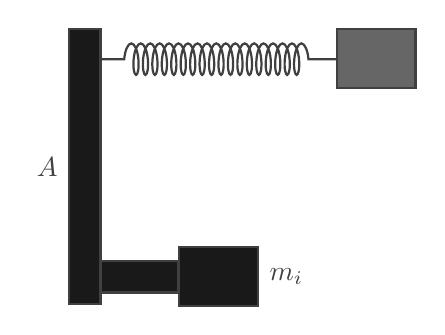
\begin{tikzpicture}[black!75,thick]

        % Supporting structure
        \node[draw,
            fill=black!90,
            minimum width=0.4cm,
            minimum height=3.5cm,
            anchor=north,
            label=west:$A$] at (-0.2,0.4) {};

        % Spring 
        \draw
        [
            decoration={
                coil,
                aspect=0.3, 
                segment length=1.2mm, 
                amplitude=2mm, 
                pre length=3mm,
                post length=3mm},
            decorate
        ] (0,0) -- ++(3,0); 


        % Mass
        \node[draw,
            fill=black!60,
            minimum width=1cm,
            minimum height=0.75cm,
            anchor=north] at (3.5, 0.4) {};
        
        \node[draw,
            fill=black!90,
            minimum width=0.98cm,
            minimum height=0.4cm,
            anchor=north] at (0.5, -2.55) {};
        
        \node[draw,
            fill=black!90,
            minimum width=1cm,
            minimum height=0.75cm,
            anchor=north,
            label=east:$m_i$] at (1.5, -2.37) {};
        

        \end{tikzpicture}        
    \caption{The carriage connected to a spring, \(A\) is the rod connected to another 
    cart. As we accelerate the cart, we also accelerate the carriage 
    and compress the spring until we achieve our desired compression length.}
\end{marginfigure}

If know we accelerate the cart, and thus the carriage, the spring experiences a particular deformation. We now measure 
when the spring stops compressing. And carefully mark the length \(l_0\) and the
acceleration in which we achieved for the cart of mass \(m_1\), \(a_1\). 

Now, we can repeat this experiment for a cart of mass \(m_2\) and get some acceleration \(a_2\)
such that by adjusting the acceleration such that the final length when it stops compressing becomes \(l_0\).

Since we claimed that the force experienced by spring is proportional to its
compression, the force experienced when a mass \(m_1\) is accelerated at \(a_1\) is 
equal to the force experienced when \(m_2\) is accelerated at \(a_2\). So, \(m_1a_1 = m_2a_2\). And
taking the \(m_1\) as the unit mass, we define,

\[m_2 \equiv m_1\frac{a_1}{a_2}.\]

We define the mass of the first body relative to the other. The accelerations
can be absolutely measured using an accelerometer. In such a manner we define 
the acceleration of any \(i\)th body relative to the first one as, 

\[m_i \equiv m_1\frac{a_1}{a_i}\]

We define some standard mass as \(1\) unit and then define the other masses 
relative to this. Such a definition is an \vocab{operational definition}.

\subsubsection{Force}

We say a \vocab{force} is produced by a physical interaction. We dont 
talk about what forces ``are''. Merely, how they come to be. Whenever 
we interact physically with an object, we apply a force on it.  

It might be tempting to ask in case of forces where such an interaction 
is not visible, say gravity, does this really hold? In fact, it does
the interaction is mediated through the use of fields. We'll have 
a look at them later.

A layman may think of forces as things that cause acceleration, that is not 
however, how a physicist views them. Thus, named forces like the 
centripetal force, are not really forces by our definition. What we do is 
we define what forces can act in a physical model. Gravity, electromagnetic force,
weak and strong force being the fundamental ones. 

Sometimes we may also be concerned with forces arising due to macroscopic effects
of small interactions. We do not thus, consider them by first principle and repeatedly 
apply the laws of our fundamental forces, but instead make empirical laws 
to avoid complexity, like the normal, tension, spring, etc. forces. 

Thus, whatever acceleration is obtained, is obtained through these forces, centripetal forces
are the components of these forces along the radial part of polar co-ordinates and not 
a force itself.

\subsection{Newton's Third Law}

The final law describes how forces come in pairs and result of a physical interaction.

\begin{axioms}
    \ii[\textbf{Axiom 3.}] If a body \(A\) applies a force on a body \(B\), then the body 
    \(B\) applies an equal and opposite force on \(A\). These forces are 
    called \vocab{action-reaction pairs}.
\end{axioms}

That is to say, 

\[\Vec{F}_{AB} = - \Vec{F}_{BA}.\]

The third law is also known as the weak law of action and reaction ---
in direct contrast with the strong law which requires the equal and opposite
forces to lie on the same line of action. Most forces such as gravity and the
normal force in fact obey the strong law of action and reaction.


\section{Some Phenomenological Forces}

\subsection{The Normal Force}

The contact force on a body can be resolved to two mutually perpendicular forces, the \vocab{normal force},
perpendicular to the object, and \vocab{friction}, tangential to the object. 

These contact forces arise due to atomic interactions. If we say keep a book on a table,
the book pushes against the table. On a microscopic scale, the molecules push against each other.
After a certain point, the molecules start repulsing each other and the table applies a normal force,
perpendicular to the body, to stop it. 

Since no object is perfectly rigid, there always occurs a deformation on its surface. However, 
this is usually negligible, and we may safely assume that the object is perfectly rigid. 

\subsection{Friction}

Friction much like the normal force, arises from molecular interactions.
It is, however, way too complex to analyse. Thus, our study of friction is 
pure phenomenological. Here, by friction we refer to dry friction, and not as is, drag. 

Friction opposes the relative motion of objects --- and this is in fact the most we 
can say safely, and generally. It is independent of the contact area.

This might feel a little weird, but consider the following argument --- say we have an object 
who has contact area with another object. This contact area is actually a very small fraction 
of its overall surface area. It is, also, proportional to the pressure.

If we double the surface area of the object, let us assume that the contact area doubles as well.
If we keep the normal force constant, the pressure halves. Friction, however, the 
product of the now half pressure, and the double contact area, remains the same.

This is a very ideal approximation of friction, but we'll make do with it now. 

We differentiate between \vocab{static friction} and \vocab{kinetic friction}. When we apply 
a force on an object, and yet it does not undergo motion, the static friction assumes a value 
to balance out the force. This friction is actually related to the normal by \(\abs{f_s} \le \mu_sN\).
Where \(\mu_s\) is the coefficient of static friction. 

However, it can not keep the object at rest forever, after a certain amount of force is applied, 
the object undergoes motion and experiences kinetic friction. It is approximately constant 
and related to the normal by \(\abs{f_k} = \mu_kN\), where \(\mu_k\) is the coefficient of kinetic friction.

Generally, \(\mu_k < \mu_s\) and they're both less than \(1\). Though for some exceptionally rough surfaces, they
may have a value greater than \(1\).

\begin{marginfigure}
    \scalebox{1}{\incfig{spinning terror}}
\end{marginfigure}

\begin{example}
    Consider a person along the wall standing inside vertical drum, of radius \(r\), in which the floor is slowly falling 
    away. If the coefficient of friction between the wall and person is \(\mu\), find 
    the smallest value of the angular speed, \(\omega\) such that the person does not fall away.

    \begin{soln}
        This is a particularly famous amusement park ride, called the spinning terror. Using
        polar co-ordinates, and that the friction must be equal to the weight to prevent slipping,
        \begin{align*}
            f &= mg \\
            N &= m\omega^2r
        \end{align*}
        
        Since \(f \le \mu N\),

        \begin{equation*}
            g \le \mu \omega^2 r \iff \omega \ge \sqrt{\frac{g}{\mu r}}
        \end{equation*}
        
    \end{soln}
\end{example}

\subsection{Tension}

\begin{marginfigure}
    \scalebox{2}{\incfig{tension,rope}}
    \caption{\(F_A\), the tension at \(A\), and \(F_B\) the tension at \(B\).}
\end{marginfigure}

The tension is the force a piece of string applies on another. Such a force 
is applied due to molecular interactions, when we stretch a string, the attraction 
between molecules opposes such a stretch and each piece of string applies tension on one another.

If the string could be compressible however, we would have had another layer of complexity,
the fact that we can bring the molecules close till only a certain distance after which 
they will start repelling each other and tension would oppose the compression.

So tension at any point is really the magnitude of force acting between adjacent sections of a rope.

\begin{marginfigure}
    \scalebox{2}{\incfig{tension,rigid}}
    \caption{Tension applied on a body connected rigidly to a pulley.}
    \label{fig: rigid tension}
\end{marginfigure}

We will shortly consider pulleys as well. If the pulleys are connected rigidly to 
a body, and a string is wrapped around it, the tension experienced by the string applies on the 
pulley as well. And since the pulley is connected through a rigid support to a body, 
it applies on the body as well. Look at \cref{fig: rigid tension}. In particular note that 
the tension on the body is directed towards the extension of the strings.

\begin{example}
    Let the rope of uniform mass density, \(\lambda\) and length \(L\) hang from a tree. Write the tension as 
    a function of position from the bottom. 
    \begin{soln}
        Consider an infinitesimal section of the rope, of length \(\dd{x}\). Since 
        the rope isn't accelerating, the net tension on the rope must balance its weight.
        Thus,
        \begin{equation*}
            T(x + \dd{x}) - T(x) = \dd{T} = \dd{m} g
        \end{equation*}

        Using \(\lambda = \dv*{m}{x} \iff \dd{m} = \lambda \dd{x}\),

        \begin{equation*}
            \int_{T}^{T_0} \dd{T} = \int_0^{L-x} \lambda g \dd{x}
        \end{equation*}

        Which is a differential equation. To solve, it we need to find \(T_0\), 
        a boundary value condition. However, note that at \(x = 0\), 
        the tension must balance the rope's weight, hence, \(T_0 = mg = \lambda Lg\).

        So we get the desired expression, \begin{equation*}
            T = \lambda xg
        \end{equation*}
    \end{soln}
\end{example}

\section{Constraints}

Sometimes the equation \(F = ma\) doesn't have all the information we need to solve a 
problem. This is often when there are constraints involved in the problem which give 
additional information.

\begin{marginfigure}
    \scalebox{2.3}{\incfig{wedge constraint}}
\end{marginfigure}

\begin{example}
Consider a block placed on a wedge. Let the wedge accelerate 
at some horizontal acceleration. Then find the relation between the accelerations 
of the block and the wedge.

\begin{soln}
    If the position of the front end of the block is 
    \((x,y)\) and that of the wedge is \((X, Y)\), 

    \begin{equation*}
        \tan\theta = \frac{Y-y}{x - X} \iff (X - x)\tan\theta = Y - y
    \end{equation*}

    Differentiating this twice with respect to time, 

    \begin{equation}
        \nddiv{y} = (\nddiv{X} - \nddiv{x}) \tan\theta
    \end{equation}

    where \(\nddiv{X}\) is the horizontal acceleration of the wedge.
\end{soln}
\end{example}

Now we will consider a rather classic system for the use of constraints,
Atwood's machine. As show in \cref{fig: atwood 1}, it is a system consisting of a pulley 
and two masses. 

\begin{marginfigure}
    \scalebox{2}{\incfig{atwood 1}}
    \caption{Classic Atwood's machine}
    \label{fig: atwood 1}
\end{marginfigure}

If we were to try and find the acceleration of the two masses, we would encounter 
three unknowns, \(a_1, a_2\) and \(T\) and two equations from the second law.

To solve such a system we can consider the vertical positions of the blocks. The idea 
here is to use the fact that a string has a fixed length(an inextensible one, anyway, but 
this is quite a forgiving approximation). If the height of the pulley is \(h\), 
their vertical accelerations \(y_1\), \(y_2\) and the length of string \(l\), then,

\begin{equation*}
    h - y_1 + h - y_2 = l
\end{equation*}

Differentiating twice with respect to time, 

\begin{equation*}
    - a_1 - a_2 = 0 \iff a_1 = -a_2
\end{equation*}

Hence, now our unknowns reduce from three to two and the system becomes solvable.
If the pulley itself was accelerating, its height was changing,

\begin{equation*}
    \nddiv{h} - a_1 + \nddiv{h} - a_2 = 0 \iff \nddiv{h} = \frac{a_1 + a_2}{2}
\end{equation*}

And generally a pulley's position is the average of the position of the masses attached to it.
If the system of pulleys consists of a lot of pulleys, it is difficult to use 
the fact that the length of the string is constant (often called the conservation of 
the string.). So we use a result from energy, that we will not derive quite yet, that is,

\begin{equation*}
    \sum Tx = \sum Tv = 0
\end{equation*}

the velocity sum is just a corollary of the position one. In a lot of scenarios, 
this can be extended to accelerations as well, but sometimes, especially when 
changing angles are involved, one needs to be careful. When such angles are not 
involved, we can easily figure out the relation between accelerations. 

For instance in our previous example,

\begin{equation*}
    Ta_1 + Ta_2 = 0 \iff a_1 = -a_2
\end{equation*}

which is the desired result.
